\chapter{Sóng, các mode lượng tử hóa và toán tử tạo}

\section{Sóng, trường và các hàm mũ phức}

Lý thuyết trường lượng tử là công cụ cơ bản của vật lý hạt. Trước khi trình bày dù chỉ ở mức sơ cấp về một trường lượng tử, sẽ hữu ích nếu tập hợp lại các kết quả toán học kết nối sóng với hạt. Bản thân sóng đã là một cấu hình trường: một trường biến thiên từ điểm này sang điểm khác trong không gian, và sóng là một cấu hình trong đó các giá trị ấy dao động và lan truyền. Cơ học lượng tử cung cấp mối liên hệ giữa những sóng như vậy và các hạt.

Ở đây giả thiết người đọc đã có nền tảng về cơ học lượng tử và thuyết tương đối hẹp. Mục đích trước mắt là ôn lại những mảnh ghép cần cho vật lý hạt, chứ không thay thế một khóa học về bất kỳ môn nào trong hai môn đó.

Hàm mũ được đặc trưng bởi sự tăng trưởng tỉ lệ. Nếu
\begin{equation}
f(x)=e^{\alpha x},
\end{equation}
thì
\begin{equation}
\frac{df}{dx}=\alpha f.
\end{equation}
Trên một khoảng nhỏ, độ tăng tỉ lệ với lượng đã có sẵn. Một quần thể tăng trưởng trong đĩa Petri cho hình dung quen thuộc: càng có nhiều sinh vật hiện diện thì càng có nhiều cá thể có thể sinh sản, nên tốc độ tăng tỉ lệ với chính quần thể đó. Nhân \(e^{\alpha x}\) với một hằng số chung không làm thay đổi tính chất đặc trưng này.

Sin và cos dao động thay vì tăng trưởng. Chúng là cùng một đường cong nhưng lệch nhau một phần tư chu kỳ, và phép đạo hàm quay chúng thành nhau:
\begin{align}
\frac{d}{dx}\sin(kx)&=k\cos(kx),\\
\frac{d}{dx}\cos(kx)&=-k\sin(kx).
\end{align}
Mỗi hàm riêng lẻ đều không phải là một hàm mũ, vì đạo hàm của nó tỉ lệ với hàm kia. Tổ hợp phức thì có tính chất hàm mũ. Với \(i^2=-1\),
\begin{align}
\frac{d}{dx}\bigl(\cos(kx)+i\sin(kx)\bigr)
&=-k\sin(kx)+ik\cos(kx)\\
&=ik\bigl(\cos(kx)+i\sin(kx)\bigr).
\end{align}
Do đó
\begin{equation}
e^{ikx}=\cos(kx)+i\sin(kx).
\end{equation}
Đồng nhất thức này xuất hiện lặp đi lặp lại vì sin và cos mô tả các dao động dạng sóng. Khi \(x\) là một tọa độ không gian, hàm dao động theo không gian. Khi đối số là thời gian, nó dao động theo thời gian.

\section{Tần số, bước sóng và động lượng của photon}

Tần số thông thường \(f\) là số chu kỳ trọn vẹn trong mỗi giây. Một chu kỳ nghĩa là một dao động đầy đủ. Tần số góc đo cùng chuyển động ấy bằng radian trên giây:
\begin{equation}
\omega=2\pi f.
\end{equation}
Hai ký hiệu này mô tả cùng một tần số. Người ta chuyển qua lại giữa chúng để tránh đưa những thừa số \(2\pi\) không cần thiết vào phép tính, dù các thừa số ấy không bao giờ biến mất hoàn toàn.

Bước sóng \(\lambda\) là quãng đường chiếm bởi một chu kỳ không gian hoàn chỉnh. Nếu một sóng lan truyền với tốc độ \(v\), thì quãng đường trên mỗi chu kỳ nhân với số chu kỳ mỗi giây chính là tốc độ lan truyền:
\begin{equation}
\lambda f=v.
\end{equation}
Đối với ánh sáng trong chân không, \(v=c\), nên
\begin{equation}
\lambda f=c.
\end{equation}
Đối với sóng âm, vế phải là tốc độ âm thanh; còn đối với sóng nước, đó là tốc độ sóng nước thích hợp. Vì vậy, sự xuất hiện của \(c\) là một phát biểu về ánh sáng, chứ không phải một định nghĩa chung cho mọi sóng.

Cơ học lượng tử đưa vào hằng số Planck dưới hai ký hiệu,
\begin{equation}
\hbar=\frac{h}{2\pi}.
\end{equation}
Việc đổi từ \(h\) sang \(\hbar\) chỉ đơn thuần chuyển các thừa số \(2\pi\) từ phương trình này sang phương trình khác.

Giá trị số của các hằng số có thứ nguyên phụ thuộc vào hệ đơn vị dùng để biểu diễn chúng. Mét, giây và kilôgam là những quy ước theo thang kích thước của con người, thuận tiện cho các độ dài và thời gian thông thường. Các đơn vị truyền thống cỡ chiều dài một cánh tay từng hữu ích cho vải hoặc dây; dù con đường lịch sử chính xác dẫn đến mét là gì, không có nguyên lý cơ bản nào chọn ra đúng thang kích thước con người cụ thể này. Trong đơn vị SI,
\begin{equation}
\begin{aligned}
h &\simeq 6.6\times10^{-34}\ \mathrm{J\,s},
&\hbar &\simeq 1.1\times10^{-34}\ \mathrm{J\,s},\\
c &\simeq 3\times10^8\ \mathrm{m\,s^{-1}}.
\end{aligned}
\end{equation}
Điều cốt yếu của các con số này là thang độ của chúng trong các đơn vị quy ước: hằng số Planck nhỏ một cách khác thường và tốc độ ánh sáng lớn một cách khác thường.

Một lượng tử của một mode có năng lượng
\begin{equation}
E_{\text{one quantum}}=\hbar\omega=hf.
\end{equation}
Đây là năng lượng của một photon, không phải tổng năng lượng của một sóng điện từ cổ điển bất kỳ. Ánh sáng khả kiến có tần số cỡ \(10^{15}\) chu kỳ mỗi giây, nên một photon quang học điển hình có năng lượng cỡ
\begin{equation}
E_\gamma\sim 10^{-19}\ \mathrm{J}.
\end{equation}
Ngay cả một dao động quang học nhanh như vậy cũng cho năng lượng trên mỗi lượng tử rất nhỏ vì \(h\) quá nhỏ. Vì thế, một lượng năng lượng quang học vĩ mô chứa một số photon khổng lồ.

Năng lượng và động lượng đáng được chú ý đặc biệt vì cả hai đều được bảo toàn. Chúng là những đại lượng ghi sổ hữu ích: tổng năng lượng và động lượng đi vào một quá trình phải được cân bằng bởi tổng năng lượng và động lượng đi ra khỏi nó. Động lượng là một vectơ và hướng theo chiều chuyển động. Đối với một hạt chuyển động chậm hơn ánh sáng rất nhiều,
\begin{equation}
\vec p=m\vec v.
\end{equation}

Bây giờ hãy xét bức xạ điện từ được chuẩn trực theo một hướng, thay vì phân tán ra nhiều hướng. Động lượng của nó hướng dọc theo chùm. Công thức phi tương đối tính không thể áp dụng cho photon, vì \(m\) nghĩa là khối lượng nghỉ và photon có khối lượng nghỉ bằng 0. Tuy vậy vẫn có một cách ghi nhớ theo thứ nguyên hữu ích. Nếu người ta gán cho photon, một cách \emph{không thích hợp}, đại lượng \(E/c^2\) như thể đó là một khối lượng rồi sau đó thế \(v=c\), thì được
\begin{equation}
mv\longrightarrow \frac{E}{c^2}c=\frac{E}{c}.
\end{equation}
Thao tác này tình cờ cho ra đáp án đúng và cho đúng đơn vị, nhưng nó không phải là một lập luận hợp lệ cho thấy photon có khối lượng nghỉ \(E/c^2\). Phát biểu tương đối tính đúng cho bức xạ được chuẩn trực theo một hướng là
\begin{equation}
|\vec p|=\frac{E}{c}.
\end{equation}
Phương trình này cho độ lớn. Hướng là hướng mà bức xạ truyền đi.

Đối với một photon,
\begin{align}
|\vec p_\gamma|
&=\frac{E_\gamma}{c}
=\frac{hf}{c}.
\end{align}
Đối với ánh sáng,
\begin{equation}
\lambda f=c,
\qquad
\frac{f}{c}=\frac{1}{\lambda},
\end{equation}
và do đó
\begin{equation}
|\vec p_\gamma|=\frac{hf}{c}=\frac{h}{\lambda}.
\end{equation}

\begin{figure}[t]
\centering
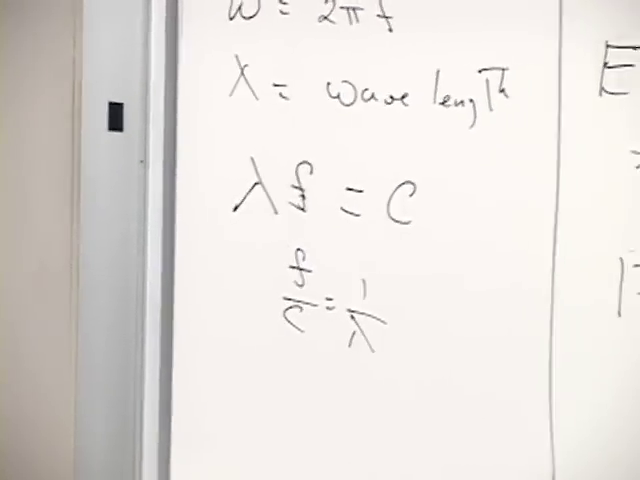
\includegraphics[width=0.56\textwidth]{lecture_02_figure_02.png}
\caption{Đối với ánh sáng, \(\lambda f=c\) và \(f/c=1/\lambda\) là các hệ thức dùng để suy ra \(|\vec p_\gamma|=h/\lambda\).}
\lectureframe{00:21:39}
\end{figure}

Bước sóng càng ngắn thì động lượng photon càng lớn. Đây là một trong những sự kiện lượng tử quan trọng nhất đối với vật lý hạt. Muốn nghiên cứu một vật nhỏ thì cần một đầu dò có bước sóng ngắn, và cái giá của bước sóng ngắn ấy là động lượng lớn.

\begin{classroomqa}
\lecturetimestamp{00:22:23}
\audiencequestion{Liệu \(E=\hbar\omega\) là cơ bản, hay được suy ra từ một nguyên lý sâu hơn?}
\lecturerresponse{Nó suy ra từ cơ học lượng tử của dao động tử điều hòa. Ở đây sẽ dùng kết quả đó mà không lặp lại chứng minh của nó; ngôn ngữ dao động tử được phát triển bên dưới cho bối cảnh sâu hơn của kết quả ấy.}
\end{classroomqa}


\section{Biên độ sóng và số photon}

\begin{classroomqa}
\lecturetimestamp{00:23:10}
\audiencequestion{Biên độ của một sóng có nghĩa gì trong ngôn ngữ photon?}
\lecturerresponse{Hãy so sánh hai sóng có cùng bước sóng và tần số nhưng biên độ khác nhau, chẳng hạn \(\sin(kx)\) và \(A\sin(kx)\). Theo cổ điển, năng lượng trong một vùng cố định tỉ lệ với bình phương biên độ. Theo lượng tử, một mode chứa \(n\) photon có năng lượng \(n\hbar\omega\). Vì vậy, khi giữ cố định tần số, vùng xét và chuẩn hóa, biên độ tăng theo bậc độ lớn như \(\sqrt n\).}
\end{classroomqa}

Hai sóng này giống hệt nhau về dạng dao động. Chỉ là một sóng mạnh hơn sóng kia.\footnote{Sơ đồ này theo phép so sánh sóng tại 00:23:47--00:24:28.}

\begin{figure}[t]
\centering
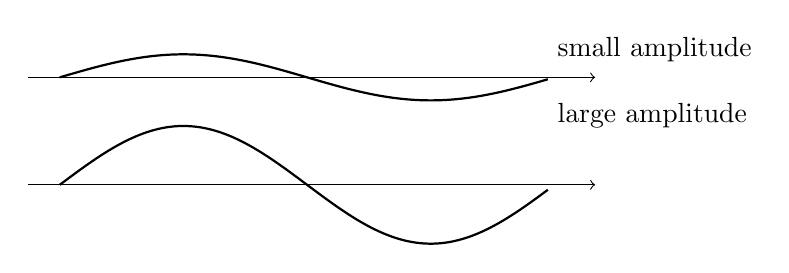
\begin{tikzpicture}[x=1cm,y=0.65cm]
\draw[->] (-0.4,0) -- (6.8,0);
\draw[->] (-0.4,-2.1) -- (6.8,-2.1);
\draw[thick] plot[domain=0:6.2,samples=120] (\x,{0.45*sin(\x r)});
\draw[thick] plot[domain=0:6.2,samples=120] (\x,{-2.1+1.15*sin(\x r)});
\draw (6.2,0.55) node[right]{small amplitude};
\draw (6.2,-0.75) node[right]{large amplitude};
\end{tikzpicture}
\caption{Các sóng có cùng bước sóng và tần số nhưng biên độ khác nhau.}
\end{figure}

Với một lượng sóng cố định,
\begin{equation}
E_{\text{wave}}\propto A^2.
\end{equation}
Đối với sóng điện từ, đây là phát biểu quen thuộc rằng năng lượng trường tỉ lệ với bình phương cường độ trường. Nếu cùng mode đó chứa \(n\) photon, thì
\begin{equation}
E_{\text{wave}}=n\hbar\omega.
\end{equation}
Do đó, khi giữ cố định mode, tần số, chuẩn hóa và vùng xét,
\begin{equation}
A^2\propto n\hbar\omega,
\qquad
A\propto\sqrt n\quad\text{at fixed }\omega.
\end{equation}
Ở đây không hề khẳng định một quy ước chuẩn hóa chính xác nào. Bao nhiêu phần của sóng được tính vào là điều quan trọng: gấp đôi chiều dài của một sóng đồng đều về mọi mặt khác sẽ làm thay đổi tổng năng lượng của nó mà không làm thay đổi biên độ cục bộ. Vì thế, phép tỉ lệ này có thể được hiểu cho một vùng cố định, chẳng hạn một bước sóng.

Cũng có một bảo lưu riêng của cơ học lượng tử. Biên độ và pha không thể đồng thời được gán các giá trị cổ điển chính xác. Vì thế câu hỏi ``Biên độ của một photon là bao nhiêu?'' là mơ hồ nếu nó đòi hỏi một trường cổ điển được xác định hoàn toàn. Tuy vậy, đặt \(n=1\) vẫn cho một thang bậc độ lớn hợp lý.

\begin{classroomqa}
\lecturetimestamp{00:28:25}
\audiencequestion{Độ lệch thẳng đứng trong một hình vẽ sóng điện từ có biểu diễn vị trí của photon trong không gian không?}
\lecturerresponse{Không. Trục lan truyền là trục không gian, còn tọa độ thẳng đứng biểu diễn giá trị của trường điện hoặc trường từ. Động lượng hướng dọc theo trục lan truyền, không dọc theo biên độ trường được vẽ ra.}
\end{classroomqa}

Sóng có thể lan truyền theo bất kỳ hướng không gian nào, nhưng hình sin quen thuộc chỉ dùng trục ngang của nó làm một tọa độ không gian. Hướng còn lại trên hình ghi lại cường độ trường.

\begin{classroomqa}
\lecturetimestamp{00:29:37}
\audiencequestion{Số photon được nêu đang được đếm trong một bước sóng hay một chu kỳ của sóng?}
\lecturerresponse{Ta có thể chọn một vùng cố định, chẳng hạn một bước sóng. Đó là lý do quan hệ chỉ là tỉ lệ: tổng năng lượng và số photon còn phụ thuộc vào việc lấy bao nhiêu phần của sóng vào. 2, 3 hoặc 4 bước sóng tương ứng chứa nhiều năng lượng hơn 1 bước sóng ở cùng biên độ.}
\end{classroomqa}

\begin{classroomqa}
\lecturetimestamp{00:30:17}
\audiencequestion{Biên độ của một photon đơn lẻ có vô nghĩa không?}
\lecturerresponse{Nó chỉ có ý nghĩa như một phát biểu về bậc độ lớn thu được bằng cách đặt \(n=1\). Đối với một mode điện từ, thông tin về điện trường và từ trường đóng vai trò tương tự như thông tin liên hợp về vị trí và động lượng, nên độ bất định lượng tử giới hạn mức độ sắc nét mà người ta có thể gán cho một biên độ cổ điển. Quan hệ ở mức bậc độ lớn vẫn hữu ích.}
\end{classroomqa}

Những câu hỏi này đã dẫn vào lý thuyết trường lượng tử, nơi mối liên hệ giữa các biến trường và số hạt có thể được phát biểu một cách chính xác. Còn hiện tại, các quan hệ tỉ lệ là đủ.

\section{Các quan hệ lượng tử tổng quát và sóng vật chất chuyển động chậm}

Một số công thức được giới thiệu cho photon áp dụng tổng quát hơn nhiều, còn những công thức khác thì không. Nên phân loại chúng trước khi chuyển sang electron.

\begin{figure}[t]
\centering
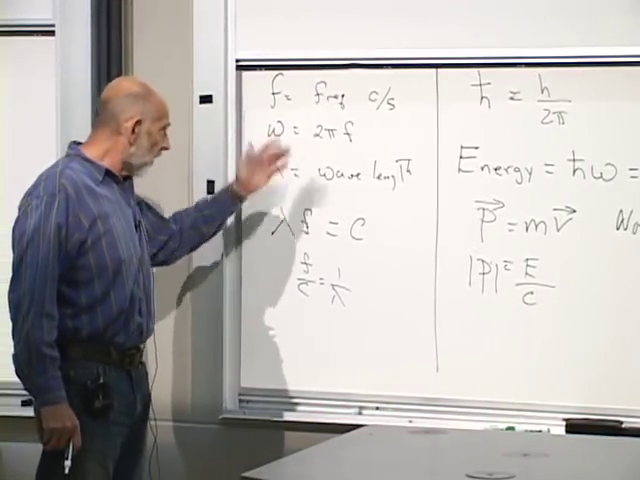
\includegraphics[width=0.82\textwidth]{lecture_02_figure_03.png}
\caption{Các định nghĩa về sóng và các hệ thức động lượng cho photon cũng như cho trường hợp phi tương đối tính, được so sánh theo miền hiệu lực của chúng.}
\lectureframe{00:31:52}
\end{figure}

Các định nghĩa của \(f\), \(\omega=2\pi f\) và \(\lambda\) áp dụng nói chung. Quan hệ lượng tử
\begin{equation}
E=\hbar\omega=hf
\end{equation}
cũng có tính tổng quát trong thảo luận hiện tại. Trái lại, các công thức chứa \(c\), chẳng hạn \(\lambda f=c\) và \(|\vec p|=E/c\), áp dụng cho các sóng chuyển động với tốc độ ánh sáng. Công thức \(\vec p=m\vec v\) áp dụng cho các hạt chuyển động chậm hơn ánh sáng rất nhiều. Chuyển động tương đối tính nằm giữa các giới hạn đó đòi hỏi một phép nội suy mà hiện chưa cần đến.

Quan hệ động lượng--bước sóng vẫn còn đúng ngoài ví dụ photon:
\begin{equation}
p=\frac{h}{\lambda}.
\end{equation}
Ở đây \(p\) ký hiệu độ lớn khi \(\lambda\) được lấy là một bước sóng dương; hướng có thể được bổ sung riêng.

\begin{figure}[t]
\centering
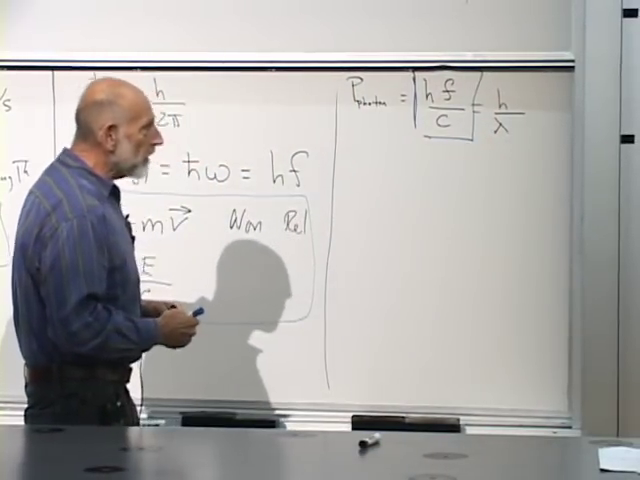
\includegraphics[width=0.74\textwidth]{lecture_02_figure_04.png}
\caption{Động lượng photon \(|\vec p_\gamma|=hf/c=h/\lambda\), dẫn đến hệ thức de Broglie tổng quát.}
\lectureframe{00:33:32}
\end{figure}

Có thể gắn một sóng với electron, hạt nhân, và thậm chí cả một quả bóng bowling. Giao thoa electron là một biểu hiện của điều đó. Ký hiệu sóng electron là \(\psi\). Đối với một electron chuyển động chậm, hệ thức nào thay thế \(\lambda f=c\)? Thành phần còn thiếu là quan hệ phi tương đối tính giữa năng lượng và động lượng.

Bắt đầu với động năng và động lượng:
\begin{align}
E&=\frac12 mv^2,\\
p&=mv,
\qquad
v=\frac{p}{m}.
\end{align}
Thế hệ thức cuối vào hệ thức đầu cho
\begin{align}
E
&=\frac12m\left(\frac{p}{m}\right)^2\\
&=\frac{p^2}{2m}.
\end{align}
Khối lượng nằm ở tử trong \(\frac12 mv^2\) và ở mẫu trong \(p^2/(2m)\). Vị trí ấy dễ nhầm lẫn, nên việc tự suy ra lại khá hữu ích.

Bây giờ dùng các quan hệ lượng tử tổng quát
\begin{equation}
E=hf,
\qquad
p=\frac{h}{\lambda}.
\end{equation}
Đối với một hạt chuyển động chậm đơn lẻ,
\begin{align}
hf
&=\frac{p^2}{2m}\\
&=\frac{1}{2m}\left(\frac{h}{\lambda}\right)^2\\
&=\frac{h^2}{2m\lambda^2}.
\end{align}
Chia cho \(h\) thu được
\begin{equation}
f=\frac{h}{2m\lambda^2}.
\end{equation}

\begin{figure}[t]
\centering
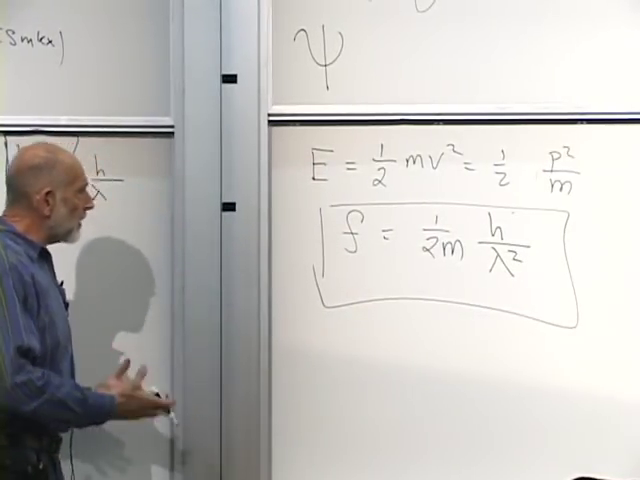
\includegraphics[width=0.64\textwidth]{lecture_02_figure_05.png}
\caption{Đối với một hạt chậm, \(E=p^2/(2m)\) và \(p=h/\lambda\) cho \(f=h/(2m\lambda^2)\).}
\lectureframe{00:37:47}
\end{figure}

Đối với ánh sáng,
\begin{equation}
f\propto\frac{1}{\lambda},
\end{equation}
trong khi đối với vật chất chuyển động chậm,
\begin{equation}
f\propto\frac{1}{\lambda^2}.
\end{equation}
Không cần phải ghi nhớ riêng lẻ hệ thức thứ hai. Luôn có thể dựng lại nó từ \(E=p^2/(2m)\), \(E=hf\) và \(p=h/\lambda\). Đối với một electron chuyển động chậm trong nguyên tử, nó cho tần số của sóng Schr\"odinger tương ứng.

\begin{classroomqa}
\lecturetimestamp{00:38:35}
\audiencequestion{Hệ thức tần số--bước sóng phi tương đối tính có áp dụng cho các hạt khác electron không?}
\lecturerresponse{Có. Nó áp dụng cho mọi hạt chuyển động chậm hơn ánh sáng rất nhiều. Phép nội suy tương đối tính giữa giới hạn chậm và giới hạn ánh sáng là một chủ đề riêng.}
\end{classroomqa}

\begin{classroomqa}
\lecturetimestamp{00:38:55}
\audiencequestion{Quan hệ nào áp dụng cho neutrino?}
\lecturerresponse{Điều đó phụ thuộc vào tốc độ của neutrino. Hầu hết neutrino gặp trong tự nhiên chuyển động rất gần tốc độ ánh sáng, nên quan hệ trong giới hạn ánh sáng là một xấp xỉ tốt. Thay vào đó, một neutrino chuyển động chậm hơn ánh sáng rất nhiều sẽ tuân theo quan hệ phi tương đối tính.}
\end{classroomqa}

\editorialnote{Một trao đổi ngắn với thính giả ngay sau câu hỏi về neutrino bàn về biên độ, lượng tử và sự khác nhau của các bước sóng electron, nhưng câu chữ bị hỏng quá nặng nên không thể phục dựng một cách chắc chắn. Phần trả lời còn khôi phục được đã hoãn việc nêu quan hệ tổng quát giữa biên độ và các lượng tử có bước sóng khác nhau.}

\begin{classroomqa}
\lecturetimestamp{00:39:56}
\audiencequestion{Một electron từ một máy gia tốc \(20\,\mathrm{keV}\) là chậm hay tương đối tính?}
\lecturerresponse{Nó được xem là chậm. Trong hệ đơn vị với \(c=1\), khối lượng, năng lượng và động lượng có thể được biểu diễn bằng cùng một đơn vị. Thang năng lượng nghỉ của electron xấp xỉ \(0.5\,\mathrm{MeV}\), còn \(20\,\mathrm{keV}\) thì nhỏ hơn nhiều. Tương đương, tiêu chuẩn động lượng phi tương đối tính là \(p\ll mc\).}
\end{classroomqa}

Phép so sánh năng lượng trong ví dụ là
\begin{equation}
K=20\,\mathrm{keV}\ll m_ec^2\simeq0.5\,\mathrm{MeV}.
\end{equation}
\editorialnote{Đoạn nguồn tại 00:39:56--00:41:40 đưa vào \(20\,\mathrm{keV}\) như một năng lượng máy gia tốc rồi diễn đạt tiêu chuẩn tương đối tính theo động lượng so với khối lượng nghỉ. Việc viết riêng tiêu chuẩn năng lượng động học và tiêu chuẩn động lượng tránh đồng nhất năng lượng được nêu với một động lượng mà vẫn giữ kết luận phi tương đối tính đã phát biểu.}

\section{Vận tốc pha, vận tốc nhóm và sự tán sắc}

\begin{classroomqa}
\lecturetimestamp{00:41:46}
\audiencequestion{Có thể dùng tích của tần số với bước sóng để suy ra vận tốc của sóng electron không?}
\lecturerresponse{Nó cho vận tốc pha, chứ không phải vận tốc gán cho electron. Một gói định xứ có cả vận tốc pha, mô tả chuyển động của các đỉnh và đáy sóng bên trong nó, lẫn vận tốc nhóm, mô tả chuyển động của đường bao. Vận tốc nhóm được đồng nhất với chuyển động của hạt.}
\end{classroomqa}

Một gói sóng, xét cục bộ, trông như một hàm sin hay cos nhưng bị giới hạn bởi một đường bao. Khi nó chuyển động, đường bao và các đỉnh sóng bên trong không nhất thiết chuyển động cùng tốc độ.\footnote{Hình minh họa này theo sau phần thảo luận về gói sóng tại 00:42:34--00:44:11.}

\begin{figure}[t]
\centering
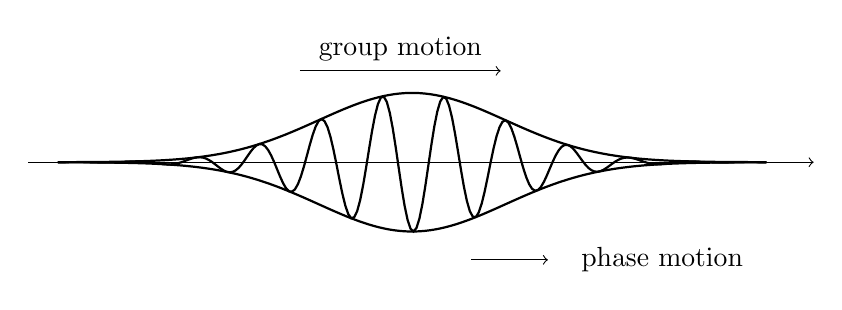
\begin{tikzpicture}[x=0.75cm,y=0.8cm]
\draw[->] (-0.5,0) -- (12.8,0);
\draw[thick] plot[domain=0:12,samples=140] (\x,{1.10*exp(-0.20*(\x-6)^2)});
\draw[thick] plot[domain=0:12,samples=140] (\x,{-1.10*exp(-0.20*(\x-6)^2)});
\draw[thick] plot[domain=0:12,samples=240] (\x,{1.10*exp(-0.20*(\x-6)^2)*sin(6*\x r)});
\draw[->] (4.1,1.45) -- (7.5,1.45);
\draw (5.8,1.8) node{group motion};
\draw[->] (7.0,-1.55) -- (8.3,-1.55);
\draw (8.7,-1.55) node[right]{phase motion};
\end{tikzpicture}
\caption{Một gói sóng định xứ mà đường bao và pha bên trong nói chung chuyển động với các vận tốc khác nhau.}
\end{figure}

Vận tốc pha là vận tốc của các đỉnh, đáy và các pha cố định khác của một thành phần đơn sắc. Đối với quan hệ tán sắc phi tương đối tính,
\begin{equation}
v_\phi=f\lambda=\frac{h}{2m\lambda}.
\end{equation}
Nó phụ thuộc vào bước sóng. Vì thế các thành phần có bước sóng khác nhau có các vận tốc pha khác nhau, nên các đỉnh sóng có thể đi xuyên qua gói và gói có thể tán ra. Vận tốc nhóm là vận tốc của toàn bộ gói, và đó là vận tốc được đồng nhất với chuyển động của hạt.

Có một trường hợp đặc biệt đơn giản. Nếu tất cả các thành phần bước sóng đều chuyển động với cùng một vận tốc, thì vận tốc pha và vận tốc nhóm trùng nhau. Ánh sáng trong chân không có tính chất này: mọi bước sóng đều truyền với \(c\). Quan hệ cho hạt chậm thì không như vậy; \(f\lambda\) của nó thay đổi theo \(\lambda\).

Phương trình
\begin{equation}
f=\frac{h}{2m\lambda^2}
\end{equation}
là phương trình Schr\"odinger tự do dưới một dạng hơi biến đổi. Tần số xác định sự phụ thuộc theo thời gian của một sóng phẳng, bước sóng xác định sự phụ thuộc theo không gian của nó, và phương trình Schr\"odinger liên hệ hai đại lượng ấy. Ngược lại, thay một sóng có tần số xác định và bước sóng xác định vào phương trình Schr\"odinger tự do sẽ tái tạo quan hệ tán sắc này.

\begin{classroomqa}
\lecturetimestamp{00:47:02}
\audiencequestion{Vận tốc pha có thể vượt quá tốc độ ánh sáng không?}
\lecturerresponse{Có. Vận tốc pha không mang thông tin. Thông tin và gói định xứ truyền với vận tốc nhóm, nên một vận tốc pha siêu quang không cho phép truyền tín hiệu siêu quang.}
\end{classroomqa}

\section{Không gian hữu hạn và động lượng rời rạc}

Mối quan tâm sau cùng là các sóng trong một không gian vô hạn, nhưng một hệ hữu hạn là điểm khởi đầu an toàn hơn. Vô hạn không phải là thứ mà máy tính có thể lưu trữ hay thao tác trực tiếp. Trước hết người ta thiết lập các phương trình cho một hệ hữu hạn rồi chỉ sau đó mới lấy giới hạn trong đó kích thước của nó trở nên lớn tùy ý. Thói quen này hữu ích trong toàn bộ cơ học lượng tử, lý thuyết trường lượng tử và vật lý hạt.

Không mất đi điều gì cốt yếu khi bắt đầu trong một chiều không gian. Sóng có thể tồn tại trên một dây đàn violin, trên một sợi dây đang được rung, hoặc trong một thế giới một chiều trừu tượng. Hệ hữu hạn hiển nhiên nhất là một đoạn có độ dài \(L\) với hai đầu phản xạ. Một sóng truyền đến một đầu, phản xạ và truyền ngược lại. Đó là một điều kiện biên phản xạ hoàn toàn hợp lệ, nhưng có một bất tiện: động lượng không được bảo toàn trong hệ sóng. Một sóng truyền sang phải mang động lượng sang phải; sau phản xạ nó mang động lượng sang trái. Biên đã cung cấp xung lực và hấp thụ phần chênh lệch.

Sự đảo chiều động lượng ở một đầu phản xạ có thể được biểu diễn bằng sơ đồ.\footnote{Hình minh họa này theo sau lập luận về biên phản xạ tại 00:49:24--00:51:08.}

\begin{figure}[t]
\centering
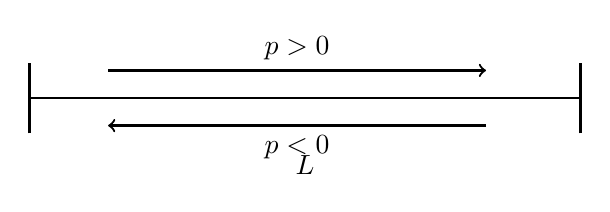
\begin{tikzpicture}[x=1cm,y=1cm]
\draw[thick] (0,0) -- (7,0);
\draw[very thick] (0,-0.45) -- (0,0.45);
\draw[very thick] (7,-0.45) -- (7,0.45);
\draw[->,thick] (1.0,0.35) -- (5.8,0.35) node[midway,above]{\(p>0\)};
\draw[->,thick] (5.8,-0.35) -- (1.0,-0.35) node[midway,below]{\(p<0\)};
\draw (3.5,-0.85) node{\(L\)};
\end{tikzpicture}
\caption{Phản xạ ở hai đầu của một đoạn hữu hạn đảo ngược động lượng của một sóng truyền.}
\end{figure}

Có một cách khác để làm cho hệ trở nên hữu hạn mà vẫn bảo toàn động lượng. Hãy đồng nhất hai đầu mút của đoạn thẳng. Có thể vẽ kết quả thành một đường tròn, nhưng không cần một đường tròn thực sự nhúng trong chiều thứ hai. Phát biểu toán học đơn giản là tọa độ có tính tuần hoàn: sau khi đi một tổng quãng đường \(L\), ta trở lại cùng một điểm.

\begin{figure}[t]
\centering
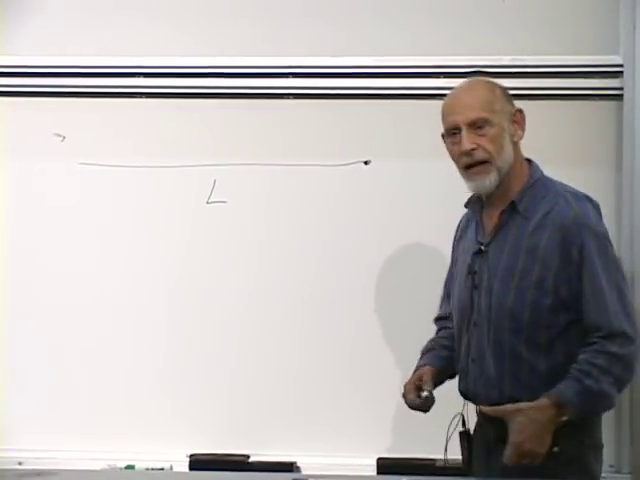
\includegraphics[width=0.72\textwidth]{lecture_02_figure_06.png}
\caption{Một đường đi một chiều có tổng độ dài \(L\) dùng để giới thiệu phép đồng nhất tuần hoàn.}
\lectureframe{00:51:21}
\end{figure}

Việc đồng nhất các đầu mút được biểu thị tường minh trong sơ đồ sau.\footnote{Hình minh họa này theo sau lập luận về phép đồng nhất tuần hoàn tại 00:51:09--00:52:37.}

\begin{figure}[t]
\centering
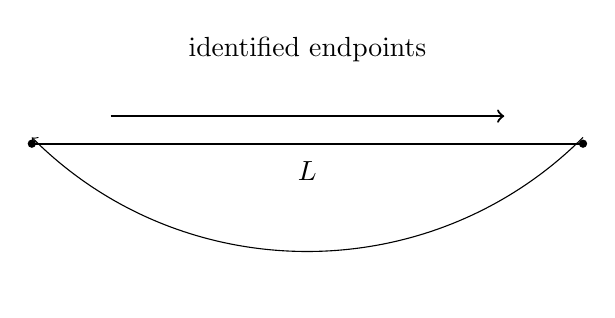
\begin{tikzpicture}[x=1cm,y=1cm]
\draw[thick] (0,0) -- (7,0);
\fill (0,0) circle (1.5pt);
\fill (7,0) circle (1.5pt);
\draw[->,thick] (1.0,0.35) -- (6.0,0.35);
\draw (3.5,-0.35) node{\(L\)};
\draw[->,bend left=45] (7,0.08) to (0,0.08);
\draw (3.5,1.2) node{identified endpoints};
\end{tikzpicture}
\caption{Không gian một chiều tuần hoàn được tạo thành bằng cách đồng nhất các đầu mút của một đường đi có độ dài \(L\).}
\end{figure}

Khi đó, một sóng chuyển động sang phải sẽ đến đầu mút được vẽ ra, xuất hiện trở lại ở điểm đầu và tiếp tục chuyển động sang phải. Tương tự, một sóng chuyển động sang trái cũng tiếp tục chuyển động sang trái. Không có đầu mút đặc biệt nào nơi sóng bị phản xạ, nên động lượng không đảo chiều. Không gian tuần hoàn làm thể tích trở nên hữu hạn và bảo toàn động lượng, nhưng nó có một hệ quả quan trọng: các động lượng cho phép là rời rạc.

Một số nguyên bước sóng phải vừa khít trong tổng độ dài. Đối với một mode không hằng,
\begin{equation}
\lambda_{|N|}=\frac{L}{|N|},
\qquad |N|=1,2,3,\ldots .
\end{equation}
Do đó độ lớn bước sóng có thể là \(L\), \(L/2\), \(L/3\), vân vân. Một lựa chọn như \(L/\sqrt{2}\) thì không khớp: sau một vòng, sóng sẽ trở về với sai pha và không trùng với giá trị ban đầu của nó.

Dùng \(p=h/\lambda\), độ lớn của động lượng đối với mode không hằng thứ \(|N|\) là
\begin{equation}
|p_N|=\frac{|N|h}{L}.
\end{equation}
Để bao gồm cả hai hướng và mode hằng mà không mơ hồ, tiện nhất là cho nhãn mode mang dấu:
\begin{equation}
p_N=\frac{Nh}{L},
\qquad N=0,\pm1,\pm2,\ldots .
\end{equation}
Các \(N\) dương và âm mô tả các hướng truyền ngược nhau. Mode \(N=0\) là hằng và có động lượng bằng không; nó không có bước sóng hữu hạn để thế vào \(h/\lambda\). Vì vậy khoảng cách động lượng cơ bản là \(h/L\).

Đối với một \(L\) vĩ mô, cả \(h\) lẫn \(1/L\) đều làm cho khoảng cách này cực nhỏ, nên các giá trị cho phép tạo thành một tập rất dày và trông gần như liên tục. Tuy vậy, một hạt cườm bị ràng buộc trên một vòng dây tròn vẫn có đúng phổ rời rạc như thế.

\begin{classroomqa}
\lecturetimestamp{00:58:27}
\audiencequestion{Đại lượng bị lượng tử hóa là tổng động lượng của sóng, hay động lượng gắn với một chu kỳ?}
\lecturerresponse{Phát biểu này áp dụng cho động lượng của mỗi lượng tử. Mỗi lượng tử có một trong các động lượng rời rạc cho phép. Do đó tổng động lượng của bất kỳ tập hợp lượng tử nào cũng là một bội số nguyên của đơn vị cơ bản \(h/L\).}
\end{classroomqa}

\begin{classroomqa}
\lecturetimestamp{00:59:22}
\audiencequestion{Vì sao sóng phải trở về cùng một giá trị sau một vòng?}
\lecturerresponse{Các đầu mút đã được đồng nhất là cùng một điểm vật lý, nên một trường quan sát được phải có cùng giá trị tại đó. Một sự không khớp sẽ đòi hỏi một bước nhảy đột ngột của trường tại điểm ấy. Sự gián đoạn như vậy là tốn kém về năng lượng và động lượng; các cấu hình trường chấp nhận được là liên tục và tuần hoàn.}
\end{classroomqa}

\begin{classroomqa}
\lecturetimestamp{01:00:09}
\audiencequestion{Điều gì xảy ra nếu sóng được định xứ thành một gói?}
\lecturerresponse{Một gói là một tổng Fourier của các sóng phẳng, hay tương đương là của các hàm sin và cos. Trong không gian tuần hoàn, tổng đó chỉ có thể chứa các mode động lượng rời rạc cho phép. Vì vậy, phát biểu về lượng tử hóa là một phát biểu về các thành phần Fourier của mọi gói chấp nhận được.}
\end{classroomqa}

\begin{classroomqa}
\lecturetimestamp{01:01:01}
\audiencequestion{Có vấn đề gì không nếu độ dài tuần hoàn \(L\) trở nên cực nhỏ?}
\lecturerresponse{Khi \(L\) giảm, động lượng cơ bản \(h/L\) trở nên rất lớn. Điều đó không hàm ý một mâu thuẫn trực tiếp nào ở các độ dài vi mô thông thường, nhưng việc cố đẩy cấu trúc này đến chế độ độ dài Planck được kỳ vọng sẽ đòi hỏi vật lý mới.}
\end{classroomqa}

Giờ hãy hiểu bức tranh đường tròn theo nghĩa đen: một hạt cườm chuyển động trên một vòng dây tròn bán kính \(r\), có chu vi \(L=2\pi r\). Các động lượng tiếp tuyến cho phép của nó là
\begin{equation}
p_N=\frac{Nh}{2\pi r}=\frac{N\hbar}{r}.
\end{equation}
Đối với một hạt phi tương đối tính trên quỹ đạo tròn, mômen động lượng là \(mvr\). Vì \(p=mv\) trong chế độ đó, đại lượng này là \(rp\). Biểu thức \(mvr\) không có tính tổng quát tương đối tính, vì khi đó \(p\) không còn đơn giản là \(mv\), nhưng động lượng nhân với khoảng cách vuông góc vẫn là quan hệ đúng. Dưới dạng vectơ,\footnote{Bài giảng lúc đầu dùng \(L\) cho mômen động lượng, rồi nhận ra sự xung đột của nó với \(L\) cho độ dài tuần hoàn và đổi ký hiệu. Ở đây dùng \(J\) xuyên suốt; xem 01:03:40--01:05:21.}
\begin{equation}
\vec J=\vec r\times\vec p,
\end{equation}
và đối với chuyển động tròn theo tiếp tuyến, độ lớn của nó là \(J=rp\). Do đó
\begin{equation}
J_N=rp_N=N\hbar.
\end{equation}
Độ giãn cách của động lượng tuyến tính phụ thuộc vào kích thước của đường tròn, còn đơn vị mômen động lượng thì luôn là \(\hbar\). Có những ngoại lệ đối với quy tắc số nguyên khi có fermion; các ngoại lệ đó sẽ được để lại bàn sau.

Nhiệm vụ tiếp theo là kết nối các trường với các hạt và lượng tử một cách chính xác hơn. Điều đó đòi hỏi quay lại ngắn gọn với cơ học lượng tử của các toán tử và dao động tử điều hòa.

\section{Các mode sóng và các toán tử lượng tử}

Phần cơ học lượng tử tiếp theo tất yếu có tính trừu tượng và nhằm mục đích ôn lại. Dao động tử điều hòa là hệ cốt yếu vì sóng là một dao động. Tại một điểm cố định, điện trường, từ trường hay bất kỳ biên độ sóng nào khác đều biến thiên tuần hoàn theo thời gian; nói rằng một thành phần có tần số tức là đã nói rằng nó dao động.

Một sóng tổng quát không nhất thiết chỉ có một bước sóng. Ánh sáng gồm nhiều màu có thể trộn lẫn với nhau, và ngược lại, một lăng kính có thể tách ánh sáng hỗn hợp thành các màu thành phần của nó, như trong phép phân tích ánh sáng trắng của Newton. Mỗi thành phần có bước sóng, tần số, biên độ, năng lượng và động lượng riêng. Vì thế sóng hỗn hợp có thể được phân giải thành các lượng tử có năng lượng và động lượng khác nhau. Mỗi bước sóng xác định một tần số, và mỗi thành phần có tần số xác định hành xử như một dao động tử. Đó là lý do vì sao dao động tử điều hòa, chứ không phải một hệ lượng tử tùy ý, là khối cấu thành tự nhiên của một trường.

Các đại lượng quan sát được trong cơ học lượng tử được biểu diễn bởi các toán tử. Các toán tử có thể được cộng và nhân, nhưng khác với các số thông thường, tích của chúng không nhất thiết độc lập với thứ tự. Gọi \(A\) và \(B\) biểu diễn hai tính chất của một hệ, mỗi tính chất đều có thể đo được riêng rẽ. Chẳng hạn, \(A\) có thể biểu diễn điện trường và \(B\) một từ trường. Nếu các giá trị đo được là các số thông thường \(a\) và \(b\), thì
\begin{equation}
ab=ba.
\end{equation}
Tích bằng số của chúng không thể phụ thuộc vào thứ tự nhân. Tuy nhiên, trong cơ học lượng tử, các toán tử tương ứng thay vào đó có thể thỏa mãn \(AB-BA\neq0\).

Thoạt đầu điều này có vẻ vô nghĩa. Nếu phép đo điện trường cho ra một số và phép đo từ trường cho ra một số khác, thì nhân hai số đó theo thứ tự nào cũng phải cho cùng một kết quả. Cách tháo gỡ là: khi các tích toán tử phụ thuộc vào thứ tự, thì hai đại lượng ấy không thể được đo đồng thời. Thí nghiệm đo một đại lượng gây nhiễu cho phép đo đại lượng kia. Không có mâu thuẫn nào, vì hai giá trị số ấy không thể thu được cùng nhau.

Khi hai đại lượng có thể được đo đồng thời, các giá trị đo được của chúng là các số thông thường, và các số đó giao hoán. Vì vậy, phép kiểm tra tính đo đồng thời là giao hoán tử
\begin{equation}
[A,B]=AB-BA.
\end{equation}
Một giao hoán tử triệt tiêu có nghĩa là các đại lượng quan sát được là tương hợp; một giao hoán tử khác không có nghĩa là các phép đo tương ứng gây nhiễu lẫn nhau. Đảo thứ tự hai mục thì đảo dấu:
\begin{equation}
[B,A]=-[A,B].
\end{equation}

Đối với một hạt phi tương đối tính, ba thành phần vị trí giao hoán với nhau, và ba thành phần động lượng cũng vậy:
\begin{align}
[x,y]&=[y,z]=[z,x]=0,\\
[p_x,p_y]&=[p_y,p_z]=[p_z,p_x]=0.
\end{align}
Cả ba tọa độ có thể được xác định cùng nhau, và cả ba thành phần động lượng cũng có thể được xác định cùng nhau. Các thành phần vị trí và động lượng tương ứng không giao hoán:
\begin{equation}
[x,p_x]=[y,p_y]=[z,p_z]=i\hbar,
\end{equation}
trong khi các thành phần trộn như \([x,p_y]\) thì triệt tiêu. Việc đo một tọa độ vị trí gây cho hạt một nhiễu động ở động lượng liên hợp. Tương đương, tích của độ bất định vị trí và động lượng tương ứng được chi phối bởi \(\hbar\).

\begin{classroomqa}
\lecturetimestamp{01:16:30}
\audiencequestion{Khi chuyển từ \(x\) sang \(y\), liệu \(i\) trong giao hoán tử có nên đổi thành \(j\) không?}
\lecturerresponse{Không. Ký hiệu \(i\) luôn luôn là đơn vị ảo, căn bậc hai của âm một. Nó không phải là nhãn vectơ đơn vị Đề-các, cũng không phải một trong các ký hiệu quaternion \(i,j,k\).}
\end{classroomqa}

\begin{classroomqa}
\lecturetimestamp{01:17:24}
\audiencequestion{Có phải \(AB-BA\) có nghĩa là đo \(A\) trước rồi đến \(B\), rồi sau đó đảo ngược thứ tự đo không?}
\lecturerresponse{Không. Hai hạng đó là các tích toán tử hoặc ma trận theo hai thứ tự đại số khác nhau. Chúng không biểu thị một chuỗi phép đo theo nghĩa đen. Mối liên hệ với các phép đo không tương hợp là hệ quả của đại số toán tử, chứ không phải định nghĩa của phép nhân.}
\end{classroomqa}

\begin{classroomqa}
\lecturetimestamp{01:18:32}
\audiencequestion{Các giao hoán tử vị trí--động lượng này có áp dụng trực tiếp cho một photon không?}
\lecturerresponse{Không trực tiếp. Chúng áp dụng gọn gàng cho các hạt phi tương đối tính. Vị trí của photon khó định nghĩa hơn, nên mệnh đề tương tự đòi hỏi phải thận trọng hơn và không cần đến ở đây.}
\end{classroomqa}

\section{Dao động tử điều hòa lượng tử}

Quả nặng gắn trên lò xo, sóng âm và sóng ánh sáng đều cho các ví dụ về chuyển động dao động. Mọi dao động tử điều hòa lý tưởng đều có một tần số. Đối với lò xo, một chu kỳ trọn vẹn không chỉ đơn thuần là thời gian cần để quả nặng trở lại cùng vị trí; nó còn phải trở lại vị trí ấy với chuyển động theo cùng một chiều. Số chu kỳ hoàn chỉnh trong mỗi giây là \(f\), và \(\omega=2\pi f\).

Theo cơ học cổ điển, một dao động tử lý tưởng có thể có bất kỳ năng lượng không âm nào. Một cú đẩy nhẹ cho một năng lượng nhỏ, còn một cú đẩy mạnh hơn cho một năng lượng lớn hơn. Một lò xo thật cuối cùng sẽ gãy hoặc nóng chảy, nhưng sự lý tưởng hóa toán học có một dải liên tục các năng lượng dương. Dao động tử lượng tử thì khác: các năng lượng được phép của nó tạo thành một thang rời rạc với khoảng cách đều nhau. Chọn gốc năng lượng sao cho mức thấp nhất được gọi là 0,
\begin{equation}
E_n=n\hbar\omega,
\qquad n=0,1,2,\ldots .
\end{equation}
Các mức cách đều có thể được hình dung như sau.\footnote{Sơ đồ mức năng lượng này bám theo phần thảo luận trên bảng tại 01:21:20--01:23:56.}

\begin{figure}[t]
\centering
\begin{tikzpicture}[x=1cm,y=0.9cm]
\draw[->] (0,0) -- (0,5.35);
\draw (0,5.5) node[above]{energy};
\foreach \y/\lab in {0.6/{0},1.6/{\hbar\omega},2.6/{2\hbar\omega},3.6/{3\hbar\omega},4.6/{n\hbar\omega}}
{
  \draw[thick] (0.2,\y) -- (2.2,\y);
  \draw (-0.25,\y) node[left]{\(\lab\)};
}
\draw[->,thick] (2.8,0.68) -- (2.8,1.52);
\draw (3.2,1.1) node[right]{\(a_+\)};
\draw[->,thick] (3.7,1.52) -- (3.7,0.68);
\draw (4.1,1.1) node[right]{\(a_-\)};
\end{tikzpicture}
\caption{Các mức của dao động tử cách đều theo quy ước \(E_n=n\hbar\omega\).}
\end{figure}

Khoảng cách \(\hbar\omega\) chính là năng lượng đã được gán trước đó cho một photon có tần số góc \(\omega\). Giá trị \(2\hbar\omega\) có thể là năng lượng của một lượng tử thuộc về một dao động tử có tần số \(2\omega\), hoặc là năng lượng của hai lượng tử trong một dao động tử có tần số \(\omega\). Cách hiểu thứ hai là cách cần dùng ở đây. Một dao động tử đơn lẻ có tần số cố định có thể chứa 0, 1, 2, 3 hoặc nhiều lượng tử hơn, và không có mức năng lượng được phép nào nằm giữa các nấc.

Số nguyên \(n\) gắn nhãn cho trạng thái của dao động tử, được viết dưới dạng ket \(|n\rangle\). Trạng thái \(|0\rangle\) là trạng thái cơ bản, \(|1\rangle\) có một lượng tử kích thích, \(|2\rangle\) có hai, v.v. Ket đơn giản chỉ là ký hiệu cho trạng thái mà các toán tử tác dụng lên.

Định nghĩa toán tử nâng \(a_+\) đưa một trạng thái lên một mức và toán tử hạ \(a_-\) đưa nó xuống một mức:
\begin{align}
a_+|n\rangle &= \sqrt{n+1}\,|n+1\rangle,\\
a_-|n\rangle &= \sqrt{n}\,|n-1\rangle.
\end{align}
Các hệ số căn bậc hai bằng số là một phần của các định nghĩa. Trên trạng thái thấp nhất,
\begin{equation}
a_-|0\rangle=0,
\end{equation}
vì không có trạng thái nào nằm dưới trạng thái cơ bản.

Điều quan trọng ở đây là phải phân biệt các số thông thường với các toán tử. Nhãn \(n\) và các hệ số như \(\sqrt n\) là các số thông thường; chúng giao hoán với mọi thứ. Các ký hiệu \(a_+\) và \(a_-\) là các toán tử, và thứ tự của chúng phải được giữ nguyên.

Trước hết hạ \(|n\rangle\) xuống, rồi nâng nó trở lại. Bước hạ cho
\begin{equation}
a_-|n\rangle=\sqrt n\,|n-1\rangle.
\end{equation}
Tác dụng \(a_+\) lên trạng thái thu được đưa vào thêm một hệ số \(\sqrt n\), vì việc nâng \(|n-1\rangle\) đưa nó trở lại \(|n\rangle\):
\begin{align}
a_+a_-|n\rangle
&=a_+\bigl(\sqrt n\,|n-1\rangle\bigr)\\
&=\sqrt n\,\sqrt n\,|n\rangle\\
&=n|n\rangle.
\end{align}
Do đó \(a_+a_-\) cho biết số mức. Chẳng hạn, giả sử \(|\chi\rangle\) được biết là một trạng thái riêng của toán tử số nhưng nhãn mức của nó chưa biết. Nếu
\begin{equation}
a_+a_-|\chi\rangle=q|\chi\rangle,
\end{equation}
thì hệ số bằng số thông thường \(q\) là số lượng tử trong trạng thái đó. Vì vậy tích ấy là toán tử số,
\begin{equation}
\hat n=a_+a_-,
\end{equation}
và, theo quy ước năng lượng đã chọn, Hamiltonian là
\begin{equation}
H=\hbar\omega\,a_+a_-.
\end{equation}
Thật vậy, tác dụng lên bất kỳ mức nào cũng cho \(H|n\rangle=n\hbar\omega|n\rangle\).

Bây giờ đảo ngược thứ tự. Nâng trước cho \(\sqrt{n+1}|n+1\rangle\). Sau đó hạ xuống thì quay về \(|n\rangle\) và đưa ra hệ số thứ hai \(\sqrt{n+1}\):
\begin{align}
a_-a_+|n\rangle
&=a_-\bigl(\sqrt{n+1}\,|n+1\rangle\bigr)\\
&=\sqrt{n+1}\,\sqrt{n+1}\,|n\rangle\\
&=(n+1)|n\rangle.
\end{align}
Hai thứ tự ấy khác nhau một đơn vị trên mọi trạng thái, nên
\begin{equation}
[a_-,a_+]=a_-a_+-a_+a_-=1.
\end{equation}

Dao động tử còn có biên độ và pha. Pha của nó cho biết nó đang ở đâu trong chu trình; cụ thể, có thể cố định pha bằng thời điểm mà dao động tử đi qua gốc theo một chiều đã chọn. Việc làm trễ lần đi qua đó làm đổi pha mà không làm đổi tần số. Các toán tử bậc thang kết hợp các biến lượng tử gắn với biên độ và pha. Đại số của chúng vốn dĩ là lượng tử, nhưng tác dụng của chúng thì đơn giản: \(a_+\) thêm một lượng tử năng lượng của dao động tử và \(a_-\) lấy đi một lượng tử. Đối với một mode điện từ, các lượng tử đó là photon, nên hai toán tử này được gọi là toán tử tạo và toán tử hủy.

\begin{classroomqa}
\lecturetimestamp{01:37:34}
\audiencequestion{Các toán tử nâng và hạ có tương ứng với một phép đo vật lý không?}
\lecturerresponse{Số photon thì đo được. Các toán tử \(a_+\) và \(a_-\) tự chúng không phải là các đại lượng quan sát được có thể đo riêng rẽ, vì những lý do kỹ thuật bổ sung. Giao hoán tử của chúng cho thấy hai toán tử đó không giao hoán, nhưng riêng sự kiện ấy tự nó không phải là lập luận cho thấy từng toán tử một, xét riêng lẻ, là không quan sát được.}
\end{classroomqa}

Một tập hợp các lò xo với các tần số riêng khác nhau cho ta nhiều dao động tử độc lập. Các mode điện từ của một hốc cộng hưởng cũng vậy: một bước sóng có thể được kích thích mà không buộc những bước sóng khác phải có cùng mức kích thích. Về mặt lượng tử, các toán tử tạo và hủy thêm vào và lấy đi các lượng tử có tần số cố định trong từng dao động tử độc lập. Ngôn ngữ này là then chốt vì các hạt sẽ được đồng nhất chính với những lượng tử đó.

\section{Một trường như một tập hợp các dao động tử}

Quay lại không gian một chiều tuần hoàn có tổng chiều dài \(L\). Các mode không hằng của nó có độ lớn bước sóng
\begin{equation}
\lambda_N=\frac{L}{N},
\qquad N=1,2,3,\ldots ,
\end{equation}
và các tần số góc không âm tương ứng \(\omega_N\). Để so sánh với phổ động lượng đã nêu trước đó, sẽ hữu ích nếu đổi nhãn số nguyên có dấu thành \(M\):
\begin{equation}
p_M=\frac{Mh}{L},
\qquad M=0,\pm1,\pm2,\ldots .
\end{equation}
Dấu của \(M\) ghi lại hướng truyền.
\editorialnote{Trong khoảng 01:42:08--01:42:24, chỉ số mode theo tần số được sửa từ một dải có dấu thành một dải chạy từ 0 trở lên. Ký hiệu \(M\) ở đây chỉ được dùng để tách biệt ký hiệu động lượng có dấu khỏi nhãn mode theo tần số không âm \(N\); nó không đưa vào các số chiếm đóng độc lập cho \(+M\) và \(-M\). Danh sách các dao động tử không hằng bắt đầu tại \(N=1\).}

Mỗi tần số được phép hành xử như một dao động tử điều hòa. Năng lượng có thể được thêm một cách độc lập vào tần số này rồi vào tần số khác. Ví dụ chi tiết đầu tiên về một trường lượng tử được để sang bài giảng tiếp theo, nhưng ký hiệu trạng thái thì đã rõ. Sắp các mode không hằng theo thứ tự từ bước sóng dài nhất trở đi, ta viết
\begin{equation}
|n_1,n_2,n_3,\ldots\rangle,
\end{equation}
trong đó \(n_N=0,1,2,\ldots\) là số lượng tử trong dao động tử có tần số \(\omega_N\). Thành phần thứ nhất cho biết có bao nhiêu lượng tử chiếm mode có bước sóng dài nhất, thành phần thứ hai cho biết có bao nhiêu lượng tử chiếm mode kế tiếp, và cứ thế mãi không dứt.

Các họa âm của một sợi dây làm cho cách xây dựng này trở nên cụ thể. Sự chuyển tiếp từ mode cơ bản qua hai họa âm tiếp theo được biểu diễn bằng sơ đồ.\footnote{Sơ đồ này bám theo phần thảo luận về các họa âm của dây tại 01:45:20--01:47:46.}

\begin{figure}[t]
\centering
\resizebox{\linewidth}{!}{%
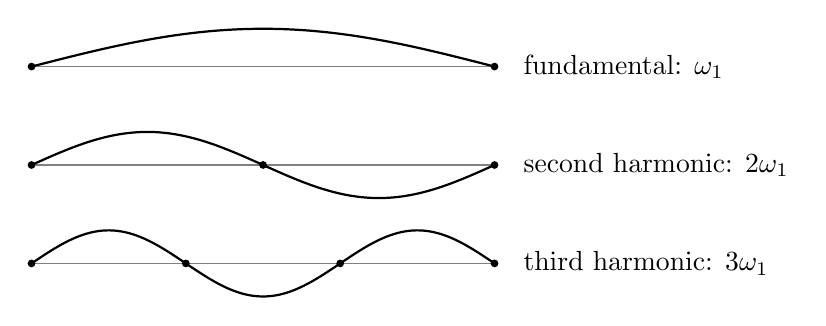
\begin{tikzpicture}[x=0.98cm,y=1cm]
\draw[gray] (0,2.5) -- (6,2.5);
\draw[thick] plot[domain=0:6,samples=120] (\x,{2.5+0.48*sin(30*\x)});
\fill (0,2.5) circle (1.4pt);
\fill (6,2.5) circle (1.4pt);
\node[right] at (6.25,2.5) {fundamental: \(\omega_1\)};

\draw[gray] (0,1.25) -- (6,1.25);
\draw[thick] plot[domain=0:6,samples=120] (\x,{1.25+0.42*sin(60*\x)});
\fill (0,1.25) circle (1.4pt);
\fill (3,1.25) circle (1.4pt);
\fill (6,1.25) circle (1.4pt);
\node[right] at (6.25,1.25) {second harmonic: \(2\omega_1\)};

\draw[gray] (0,0) -- (6,0);
\draw[thick] plot[domain=0:6,samples=120] (\x,{0.42*sin(90*\x)});
\fill (0,0) circle (1.4pt);
\fill (2,0) circle (1.4pt);
\fill (4,0) circle (1.4pt);
\fill (6,0) circle (1.4pt);
\node[right] at (6.25,0) {third harmonic: \(3\omega_1\)};
\end{tikzpicture}%
}
\caption{Mode cơ bản của dây và họa âm thứ hai, thứ ba của nó, với 0, 1 và 2 nút bên trong.}
\end{figure}

Mode cơ bản dao động như một vòm rộng duy nhất và không có nút bên trong. Nó là một dao động tử, và nó có thể chứa \(n_1=0,1,2,\ldots\) lượng tử; mỗi kích thích cần \(\hbar\omega_1\). Họa âm thứ hai có một nút bên trong và tần số gấp đôi. Nếu mode cơ bản phát ra nốt đô trung, thì mode này phát ra nốt đô cao hơn một quãng tám. Nó có một số chiếm đóng độc lập \(n_2\), và mỗi lượng tử của nó cần \(\hbar\omega_2=2\hbar\omega_1\). Họa âm thứ ba có hai nút bên trong và tần số gấp 3 lần tần số cơ bản. Nó có số chiếm đóng độc lập riêng \(n_3\), và số này một lần nữa có thể là bất kỳ số nguyên không âm nào.

Xét từng mode, theo quy ước năng lượng dùng ở trên, năng lượng bằng số chiếm đóng nhân với năng lượng lượng tử. Gộp các đóng góp đó lại, ta được
\begin{equation}
E=\sum_{N=1}^{\infty} n_N\hbar\omega_N.
\end{equation}
\editorialnote{Tổng được viết tường minh này là sự gom góp đại số của các năng lượng mode đã được phát biểu riêng rẽ tại 01:44:02--01:47:46.}

Cùng một toán học của dao động tử điều hòa phải được lặp lại cho mọi mode của trường, với một toán tử tạo và một toán tử hủy cho mỗi dao động tử độc lập. Trong bức tranh sơ cấp đầu tiên này, một trường lượng tử chính là toàn bộ tập hợp ấy của các dao động tử và đại số tạo--hủy của chúng.

Ngôn ngữ này được điều chỉnh cho phù hợp với tán xạ hạt. Các lượng tử có năng lượng và xung lượng xác định đi vào một thí nghiệm, và các lượng tử có những năng lượng và xung lượng khác đi ra khỏi thí nghiệm ấy. Các hạt ban đầu được loại bỏ bởi các toán tử hủy; các hạt đi ra được đưa vào trạng thái cuối bởi các toán tử tạo ứng với các mode thích hợp.

\begin{classroomqa}
\lecturetimestamp{01:49:38}
\audiencequestion{Có phải cùng một số nguyên đang được dùng để gán nhãn mode dao động và để đếm số lượng tử trong đó không?}
\lecturerresponse{Có hai số nguyên riêng biệt. Nhãn mode \(N\) xác định dạng phân bố trong không gian; trong ví dụ về dây, số nút của nó quyết định tần số \(\omega_N\). Số chiếm chỗ \(n_N\) cho biết có bao nhiêu lượng tử có tần số đó.}
\end{classroomqa}
